% --------------------------
% ---- DECLARE PACKAGES ----
% --------------------------
\documentclass[a4paper, oneside, openright]{book}
\usepackage[T1]{fontenc} % Font encoding, T1 = it
\usepackage{lmodern}
\usepackage{multicol} % Per il frontespizio
\usepackage[utf8]{inputenc} % Input encoding
\usepackage[english,italian]{babel} % Lingua principale italiana, con parti in inglese
\usepackage{minted} % Per i blocchi di codice
\usepackage{csquotes} % Dipendenza di babel e biblatex
\usepackage{blindtext} % Generazione di paragrafi lorem ipsum
\usepackage{graphicx} % Immagini esterne

\usepackage{setspace}
\onehalfspacing % interlinea 1.5

\usepackage[parfill]{parskip} % Disabilita l'indentazione dopo essere andati a capo
\usepackage{titlesec}
\usepackage{float}
\usepackage{booktabs}
\usepackage{longtable}

% Percorso per le immagini delle sessioni
\graphicspath{{Immagini/}{Immagini/Sessioni/}}

% Diagrammi TikZ
\usepackage{tikz}
\usepackage{pgfplots}
\usepackage{pgf-pie}
\pgfplotsset{compat=1.18}
\usetikzlibrary{shapes.geometric, arrows, positioning, fit, backgrounds}
\tikzstyle{startstop} = [rectangle, rounded corners, minimum width=3cm, minimum height=1cm,text centered, draw=black, fill=red!30]
\tikzstyle{io} = [trapezium, trapezium left angle=70, trapezium right angle=110, minimum width=3cm, minimum height=1cm, text centered, draw=black, fill=blue!30]
\tikzstyle{process} = [rectangle, minimum width=3cm, minimum height=1cm, text centered, draw=black, fill=orange!30]
\tikzstyle{decision} = [diamond, minimum width=3cm, minimum height=1cm, text centered, draw=black, fill=green!30]
\tikzstyle{arrow} = [thick,->,>=stealth]

% Captions
\usepackage[font=scriptsize, skip=5pt, justification=centering]{caption}

\usepackage[backend=biber, style=numeric, backref=true, defernumbers=true]{biblatex}

\usepackage[immediate]{silence}
\WarningFilter[temp]{latex}{Command}
\usepackage{sectsty}
\DeactivateWarningFilters[temp]
\WarningFilter{microtype}{Unable to apply patch `footnote'}

\usepackage{hyperref} % Rende l'indice cliccabile
\usepackage[bottom]{footmisc} % Posiziona le footnotes alla fine della pagina
\usepackage{subcaption}

% Sperimentali
\usepackage{microtype}

% Impaginazione e margini
\usepackage[top=3.5cm,bottom=3.5cm,left=3.5cm,right=3.5cm]{geometry}
\usepackage[fontsize=12pt]{scrextend} % dimensione font

% ------------------------
% ---- DOCUMENT SETUP ----
% ------------------------
\pagestyle{plain}
\raggedbottom % Se la pagina non è completa, lascia lo spazio alla fine

\titleformat{\chapter}[display]
{\normalfont\huge\bfseries}{\chaptertitlename\ \thechapter}{10pt}{\LARGE}
\titlespacing*{\chapter}{0pt}{0pt}{20pt}
\chaptertitlefont{\fontsize{22pt}{30pt}\selectfont}

\hypersetup{ % Aspetto dei link
    colorlinks,
    citecolor=black,
    filecolor=black,
    linkcolor=black,
    urlcolor=black
}

\renewcommand{\footnotesize}{\fontsize{11pt}{13pt}\selectfont} % Imposta la dimensione del testo delle footnotes
\setlength{\footnotesep}{0.5cm} % Imposta lo spazio fra e singole footnotes
\setlength{\skip\footins}{1.5cm} % Imposta lo spazio fra il corpo e le footnotes

\DeclareUnicodeCharacter{02BC}{}

% ------------------------
% ---- DOCUMENT START ----
% ------------------------
\addbibresource{bibliography.bib} % Bibliografia
\begin{document} % Inizio documento
\hypersetup{pageanchor=false}
\frontmatter
\begin{titlepage}
\begin{figure}[!htb]
    \centering
    
\includegraphics[width=5cm]{Immagini/uninsubria-logo}
\end{figure}

\begin{center}
    \Large{\textbf{UNIVERSITÀ DEGLI STUDI DELL'INSUBRIA}}
    \vspace{3mm}
    \\ \normalsize{DIPARTIMENTO DI SCIENZE TEORICHE E APPLICATE}
    \vspace{6mm}
    \\ \normalsize{CORSO  DI STUDIO TRIENNALE  IN}
    \\  \normalsize{\textbf{INFORMATICA}}
    \vspace{13mm}
    % \\ \normalsize{Tesi  di Laurea}
\end{center}

\vspace{10mm}
\begin{center}
    \LARGE{\textbf{Migrazione e sviluppo di un'applicazione Android per l'analisi dei melanoma}}
\end{center}

\vspace*{\fill}

\begin{minipage}[t]{1\textwidth}
    \begin{multicols}{2}
    	{\normalsize{\textbf{Relatore:}}{\normalsize\vspace{1mm}
        \\ \normalsize{Prof. Ignazio Gallo }}} \\

        %{\normalsize{\textbf{Co-relatore:}}{\normalsize\vspace{1mm}
        %\\ \normalsize{Prof. Luca Verdi }}} \\
        
         %\columnbreak
         %\columnbreak

         \begin{flushright}
            {\normalsize{\textbf{Tesi di Laurea di:}}{\normalsize\vspace{1mm}
            \\ \normalsize{Gabriele Caretti}\\
            \normalsize{Matricola  756564 }}} \\
         \end{flushright}
    \end{multicols}
\end{minipage}

\begin{center}
    {\normalsize{\textbf{Anno accademico:}}{\normalsize\vspace{1mm}
    \\ \normalsize{2025/2026}}}  
\end{center}

\end{titlepage}
 % PAGINA FRONTESPIZIO
% \cleardoublepage
\thispagestyle{empty}
\vspace*{\stretch{7}}
\begin{flushright}
\itshape Lorem ipsum, dolor sit \\
amet, consectetuer adipiscing elit.  \\ \vspace{5mm}
Praesent imperdiet mi nec ante \\
donec ullamcorper, felis non sodales.
\end{flushright}
\vspace*{\stretch{2}}
\cleardoublepage % PAGINA DEDICA
\tableofcontents  % Genera l'indice
\mainmatter
\hypersetup{pageanchor=true}
\setcounter{chapter}{0} % Fa risultare l'introduzione come capitolo 0

% ------------------
% ---- CHAPTERS ----
% ------------------
%! Author = gabry
%! Date = 03/07/2026

\chapter{Introduzione}\label{ch:introduzione}

\section{Obiettivo}\label{sec:obiettivo}
Il progetto di tesi si propone di sviluppare un'applicazione mobile cross-platform, compatibile sia su piattaforme
Android che iOS, partendo dallo sviluppo di un'applicazione nativa scritta in Android Kotlin, che necessità
di una migrazione verso Kotlin Multiplatform.
L'applicazione nativa offre analisi tramite l'input di parametri dei tumori di tipo Melanoma, con metrica Melanoma TNM,
seguendo il manuale AJCC 8th Edition.
Questa sarà successivamente estesa con l'implementazione di analisi di tipo cSCC Testa-Collo, con metrica cSCC TNM, sempre seguendo
il precedente manuale AJCC 8th Edition\@.

L'obiettivo è quello di offrire uno strumento semplice e veloce per semplificare il lavoro dei medici nella fase di analisi dei tumori,
con dati sincronizzati in ambiente cloud tramite app installabili su dispositivi mobili.

Il processo di realizzazione del software è strutturata in una sequenza lineare di fasi, nello specifico:

\begin{itemize}
    \item Analisi dei requisiti;
    \item Progettazione;
    \item Sviluppo;
    \item Conclusioni;
\end{itemize}

\section{Melanoma}\label{sec:melanoma}
Il melanoma è la forma più aggressiva e pericolosa di tumore cutaneo.
Si origina dai \textit{melanociti}, cellule presenti sull'epidermide responsabili della produzione di melanina, ossia il
pigmento che ne da il colore e la protegge dai raggi solari, come ultravioletti (UVA, UVB e UVC).
Quando il DNA di queste cellule si danneggia (spesso a causa di un'eccessiva esposizione ai componenti pericolosi dei raggi solari),
i melanociti possono iniziare a moltiplicarsi in modo incontrollato, formando quindi una massa tumorale.

A livello visivo, un melanoma può manifestarsi come la comparsa di un "neo" anomalo oppure come il cambiamento di forma, colore o dimensione di uno
già esisteste.
Sebbene i melanomi rappresentino solamente una piccola percentuale di tutti i tumori cutanei, questi sono responsabili della
maggioranza dei decessi legati a tal genere di patologie.
Questo è spesso dovuto alla loro tendenza di diffondersi nei tessuti profondi e a generare metastasi in altri organi se non individuati
in tempo.

Una diagnosi precoce e precisa può quindi salvare la vita di un individuo affetto da melanoma.
In ambito clinico, questo viene valutato attraverso il \textbf{sistema di stadiazione TNM} (Tumore, LinfoNodi, Metastasi), un metodo standardizzato
ed esposto in manuali come l'AJCC 8th Edition menzionato in precedenza, che ne definiscono con importanza critica la prognosi e il piano
terapeutico del paziente.

In un panorama ampio come quello dell'oncologia dermatologica, un'altra importante manifestazione di tale patologia è il
\textbf{Carcinoma a Cellule Squamose (SCC)}.
Quest'ultimo, specialmente nei casi in cui è localizzato nel distretto testa-collo, richiede un monitoraggio costante e attento,
a causa del suo potenziale impatto distruttivo a livello funzionale ed estetico.

Questo progetto di applicazione mobile, mira quindi allo sviluppo di uno strumento di supporto digitale, che ne semplifica le fasi
di diagnosi, con classificazione, stadiazione e storico dei pazienti affetti da melanoma TNM e cSCC TNM Testa-Collo.

% \chapter{Stato Attuale}

\section{Sistemi ERP}
I sistemi \textit{ERP} (\textit{Enterprise Resource Planning}) rappresentano un elemento essenziale del sistema gestionale aziendale \cite{erpMigration},
consentendo l'integrazione dei processi di \textit{business} principali di un'azienda come: vendite, acquisti, gestione inventario, contabilità e personale.

\subsection{Evoluzione dei Sistemi Legacy al Cloud}
Nel corso degli anni, i sistemi \textit{ERP} si sono evoluti partendo da architetture \textit{on-premise} \textit{legacy}, spesso caratterizzate da un elevato
grado di personalizzazione (\textit{customization}, in Infor LN definiti come \texttt{tx}) e importanti costi di manutenzione.
Tuttavia, oggi si sta assistendo ad una transizione verso nuove soluzioni \textit{Cloud}.

% \subsection{Architetture Multitenant}
Di fatto, il modello \textit{Cloud Multitenant} oggi rappresenta l'architettura degli \textit{ERP} moderni \cite{multitenantCloud}.
Ove, una singola istanza del software e infrastruttura servono più clienti (definiti come \textit{tenant}).
Questo approccio offre scalabilità, aggiornamenti continui e ottimizzazione dei costi, ma anche grandi sfide nell'ambito
della gestione e segregazione dei dati, nonché della sicurezza, richiedendo che ogni processo di migrazione operi
secondo specifici vincoli di integrità \cite{dataMigrationStrategies}.

\section{Infor LN e CloudSuite Enterprise}
Infor LN, nato con il nome di Baan \textit{ERP}, è uno dei principali \textit{ERP} nel settore manifatturiero industriale \cite{inforLN2025} a livello internazionale.
Viene integrato all'interno della Infor \textit{CloudSuite Enterprise}, il quale offre funzionalità per la gestione della \textit{supply chain}
e produzione \cite{inforCloudsuite}.

L'interfaccia utente Web (nota come \texttt{LNUI}) permette agli utenti finali di navigare tra le diverse sessioni
tramite \textit{menu} contestuali o ricerca diretta (Figura~\ref{fig:ln_ui}).

\begin{figure}[H]
    \centering
    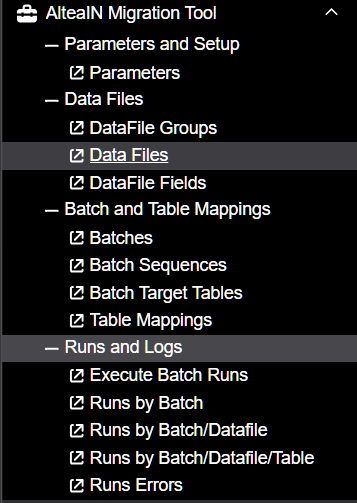
\includegraphics[width=0.5\textwidth]{Lista_Sessioni_LNUI}
    \caption{Esempio di interfaccia Web Infor LN (LNUI) con elenco sessioni del Migration Tool.}
    \label{fig:ln_ui}
\end{figure}

% \subsection{Architettura e Componenti di Infor LN}
Infor LN è basato su un'architettura che separa il \textit{framework} tecnologico (gli Infor Tools) dalla logica di \textit{business}.
Ogni applicazione è composta da diversi oggetti:
\begin{itemize}
    \item \textbf{Tabelle (\textit{Tables}):} I dati fisici, definiti tramite \textit{Data Dictionary}, con domini standard o \textit{custom}.
    \item \textbf{Sessioni (\textit{Sessions}):} Le interfacce utente (da qui definite come Sessioni) attraverso cui gli operatori accedono, visualizzano e interagiscono con i dati.
    \item \textbf{DAL (\textit{Data Access Layer}):} L'elemento che si occupa di garantire l'integrità dei dati e delle tabelle, indipendentemente dalle Sessioni \cite{inforDalGuide}.
    \item \textbf{Domini (\textit{Domains}):} Definiscono i tipi di dati, con regole di validazione e formati, che possono essere standard o personalizzati (\textit{custom}).
    \item \textbf{Etichette (\textit{Labels}):} Utilizzate per la localizzazione e la visualizzazione dei campi nelle Sessioni, con supporto multilingue (es.
    02 corrisponde alla lingua inglese, e 06 alla lingua italiano).
\end{itemize}

\subsection{Linguaggio Baan C: 3GL e 4GL}
Per lo sviluppo e personalizzazione degli \textit{script} e librerie, Infor LN utilizza un linguaggio proprietario, di nome \textbf{Baan C} \cite{infor3GL4GL}.

Esso si divide a sua volta in:
\begin{itemize}
    \item \textbf{4GL (\textit{Fourth-Generation Language}):} La versione più recente e moderna.
    Infor LN Tools genera automaticamente operazioni standard di Sessione e database (CRUD). In 4GL non è necessario
    scrivere codice per gestire il salvataggio o il caricamento di un record, ma ci si concentra sulla gestione
    degli \textit{eventi} legati ai componenti della Sessione o del database (tramite \textit{DAL} \cite{inforDal2Guide}).
    \item \textbf{3GL (\textit{Third-Generation Language}):} Precedente a 4GL, e totalmente integrato con esso, viene utilizzato
    per la gestione di logiche di \textit{business} complesse.
    Permette un approccio più procedurale e a basso livello per implementare funzioni matematiche, algoritmi personalizzati,
    \textit{DLL} (\textit{Dynamic Link Libraries}) proprietarie, funzioni e routine di manipolazione stringhe o file, nonchè di estensioni (\textit{extensions})
    che rappresentano in alcuni casi, l'unico modo di interagire e personalizzare tabelle e procedure standard.
\end{itemize}

\subsection{Infor Exchange e Strumenti di Import/Export}
Per lo scambio di informazioni, Infor fornisce un modulo denominato \textit{Exchange} \cite{inforExchangeGuide}.
Si tratta di una piattaforma per l'importazione e l'esportazione di file (es.
CSV, XML, testo a larghezza fissa)
mappando righe e colonne sui \textit{Datafiles} e sui campi del database di LN .

Spesso sono necessarie delle personalizzazioni delle procedure di migrazione tramite Baan C, che quindi risulta essenziale quando le regole di
mappatura superano la complessità gestibile nativamente dall'\textit{Exchange}.

\section{Migrazione Dati nei Sistemi ERP}
\subsection{Sfide e Problematiche Comuni}
La migrazione da un sistema \textit{legacy} a un nuovo \textit{ERP} \textit{cloud} richiede un'attenta fase di analisi per evitare perdite o
disallineamenti di informazioni storiche e \textit{master data}.

Attualmente, molte migrazioni sono gestite manualmente, con l'integrazioni di \textit{script} scritti
\textit{ad hoc}, con un alto livello di complessità e rischio d'errore.
Per questo, nasce l'idea del Tool di Migrazione (\textit{Migration Tool}) oggetto di questa tesi.

%\subsection{Migrazione verso ambienti Cloud e SaaS}
Per la migrazione verso il \textit{Cloud}, sono necessari \textit{tool} robusti in grado di lavorare sia con logiche \textit{batch} sia con \textit{API} e servizi \textit{web} (\textit{webservices} o \textit{WS} in breve),
adattandosi alle regole di \textit{business} e garantendo la qualità di ogni singolo dato prima ancora che venga scritto nel
database del nuovo \textit{tenant}.


%! Author = gabry
%! Date = 03/07/2026

\chapter{Analisi dei Requisiti}\label{ch:analisi-dei-requisiti}

Una delle prime attività fondamentali dell'ingegneria del software per la buon riuscita di un prodotto, è l'analisi dei requisiti.
Questa fase ha lo scopo di individuare e definire le funzionalità offerte che saranno sviluppate.
% Alla fine di essa sarà steso un documento di \textit{specifica dei requisiti}, che descriverà tutte queste funzionalità in modo completo e chiaro.

% Il documento di specifica dei requisiti fungerà da documento di riferimento per tutte le fasi successive dello sviluppo del software.
La nostra applicazione mobile dovrà quindi offrire:

\begin{itemize}
    \item Fase di apertura, con caricamento dell'interfaccia principale per l'inserimento dei parametri
    \item Tema dinamico, tramite pulsante per il passaggio da tema chiaro a scuro e viceversa, anche in base alle impostazioni del dispositivo
    \item Multilingua, inglese e italiano, anch'esse in base alle impostazioni del dispositivo
    \item Risultati con spiegazione delle analisi, con eventuale follow-up consigliato
    \item File di configurazione con cui definire parametricamente i risultati che gli input dovranno dare
    \item Funzionalità di salvataggio dei risultati di diagnosi dei pazienti, con possibilità di visualizzarli in uno storico con ogni loro diagnosi
    \item Funzionalità di cancellazione dei paziente, inclusi il loro storico, o delle loro singole diagnosi
    \item Funzionalità per passare da una diagnosi TNM a sSCC Testa-Collo e viceversa
    \item Funzionalità di caricamento delle diagnosi precedenti, senza dover reinserire i parametri manualmente
    \item Sincronizzazione con un servizio cloud, per salvare i dati dei pazienti e le loro diagnosi
\end{itemize}

L'app mobile deve inoltre soddisfare dei requisiti non funzionali, come:

\begin{itemize}
    \item UI/UX semplice, intuitiva e moderna, senza complicare più del necessario l'utilizzo dell'utente finale
    \item Sicurezza, sia locale che cloud
    \item Funzionalità offline, in assenza di internet l'app deve comunque permettere di eseguire diagnosi
\end{itemize}

%\chapter{Architettura}

\section{Panoramica dell'Architettura di Sistema}
L'architettura del Migration Tool è stata definita per essere modulare e scalabile.
Alla base del sistema vi è una separazione netta tra il modulo di input (Importer), il motore per l'elaborazione dei metadati,
e il Generatore di Codice.
Questo approccio garantisce una separazione tra il layout dei dati preesistenti e la struttura del database Infor CloudSuite.

\section{Progettazione del Software}
\subsection{Design dell'Importer e del Parser dei Dati}
L'Importer funge da punto d'ingresso per i dati ed è progettato per interpretare il formato proprietario di Infor Exchange,
analizzando file di esportazione testuali o strutturati.
Estraendo i metadati dai record, l'Importer popola i dizionari \textit{Datafiles} (\texttt{txamg110}) e i
relativi \textit{Fields} (\texttt{txamg111}).

Questo design del caricamento rende possibile supportare sia architetture multitenant cloud, sia installazioni legacy on-premise.

\subsection{Motore di Generazione del Codice}
Il nucleo computazionale è rappresentato dal motore di generazione.
Basato su librerie compilate (DLL come \texttt{txamgdll0012} e \texttt{txamgdll0013}), il modulo interpreta il
dizionario di mapping (definito in \texttt{txamg203} o \textit{MappedFields}) e traduce i legami e le regole di
trasformazione in script nativi Baan C.

Questo meccanismo previene di dover scrivere manualmente codice, garantendo il rispetto dei framework CloudSuite:
il codice viene prima generato, poi compilato via \texttt{bic\_compiler}, ed infine agganciato ai \textit{Batch Runs}.

\subsection{Modulo di Integrazione Ad-hoc e Callbacks}
Mentre buona parte dei flussi vengono standardizzati automaticamente, alcune regole di business richiedono sviluppi
specifici a causa della loro complessità.
Vengono quindi esposte a livello architetturale delle interfacce \textit{callback}.

In appositi \textit{module script}, gli sviluppatori possono iniettare blocchi di codice chiamati asincronamente dall'engine.
Questi script personalizzati usufruiscono degli stessi vantaggi transazionali dell'utility principale.

\section{Scelte Tecnologiche}
\subsection{Linguaggi e Framework}
L'intero ecosistema è sviluppato sfruttando l'Infor Tools Framework, programmando in \textbf{Baan C (sia 3GL che 4GL)}.
In parte sono state adottate le \textit{DAL (Data Access Layer)},
per il restante, sono state utilizzati approcci più classici e a basso livello.

\subsection{Librerie di Supporto e Strumenti di Build}
Tutto il coordinamento della configurazione, logging (\texttt{txamgdll0011}) e le \textit{string utility} si basano sulle librerie
del sistema ERP (DLL native Baan e tool come il \texttt{ttdll string}).

Le build non prevedono toolchain esterni complessi
(come Maven o MSBuild), ma si appoggiano direttamente al toolset interno dell'ERP, il quale gestisce i
legami VRC (Version Release Customer) multitenant per garantirne l'incapsulamento del codice generato al corretto Tenant.


%! Author = gabry
%! Date = 03/07/2026

\chapter{Progettazione}\label{ch:progettazione}

Successivamente alla fase di analisi dei requisiti, la fase di progettazione definisce come tali requisiti saranno
effettivamente implementati, sia a livello di struttura software che di interfaccia utente.

\section{Descrizione generale}\label{sec:descrizione-generale}

\section{Scelte architetturali}\label{sec:scelte-architetturali}

\subsection{Migrazione verso Kotlin Multiplatform}\label{subsec:migrazione-verso-kotlin-multiplatform}

Il progetto è stato inizialmente sviluppato in Kotlin nativo Android, utilizzando strumenti Java e non solo, come:

\begin{itemize}
    \item EvalEx, per la lettura dei file delle espressioni per ottenere le diagnosi
    \item Firebase, per la sincronizzazione dei dati dei pazienti e delle diagnosi
    \item SpashScreen, per l'animazione iniziale di caricamento
    \item Lingua e tema di default in base al dispositivo
\end{itemize}

Questi elementi sono stati sostituiti con altre librerie simili o sostituiti, nello specifico:

\begin{itemize}
    \item EvalEx è stato rimosso, e si è invece scritto un interprete da zero nativo Kotlin
    \item Firebase è stato sostituito con la version Gitlive della community, con l'aggiunta di diverse dipendenze per i servizi Google
    \item Lo SplashScreen animato è stato rimosso in favore di uno statico
    \item La lingua e il tema di default sono stati scritti nelle rispettive iosMain e androidMain, in quanto diverse per piattaforma
\end{itemize}

\subsection{Architettura dell'applicazione}\label{subsec:architettura-dell'applicazione}
L'architettura del software si adatta agli standard di Kotlin Multiplatform (KMP). Durante la migrazione da Kotlin a Kotlin Multiplatform, l'obiettivo primario
è stato quello di massimizzare il codice condiviso tra Android e iOS, con il minor numero di dipendenze native ove possibile, con una logica di business e di presentazione (UI) unificati.

L'applicazione segue una variante del pattern architetturale \textbf{Model-View-ViewModel (MVVM)}, costruita attorno a una singola \textit{ViewModel} centralizzata (\texttt{MelanomaViewModel}).
Questa funge da singolo punto di accesso per l'intero ciclo di vita dell'applicazione, separando l'interfaccia utente dalla logica di dominio.

Le caratteristiche architetturali principali includono:

\begin{itemize}
    \item Utilizzo di Compose Multiplaform, compatibile sia con Android che iOS in Kotlin Multiplatform, tramite
    il modulo condiviso \texttt{commonMain}.
    Le viste (View) sono \textit{stateless}, e si limitano quindi a osservare i dati e a inoltrare al ViewModel le interazioni dell'utente.
    \item Utilizzo di \texttt{StateFlow} e di \texttt{MutableStateFlow} per la gestione della reattività degli stati.
    Variabili come dati anagrafici, parametri clinici e risultati della stadiazione (\texttt{StagingResult}) vengono aggiornati reattivamente.
    Viene quindi ricomposta automaticamente l'interfaccia grafica quando i flussi di dati cambiano, emettendo un nuovo stato.
    \item Navigazione tra le schermate gestita tramite stato (State-Driven), senza librerie di routing esterne (inizialmente nella versione nativa veniva utilizzato il Navigation Component di Android), viene quindi gestita in modo manuale e dichiarativo la navigazione tra le schermate.
    Una \texttt{Sealed class Screen} definisce le possibili destinazioni navigabili dell'app (\texttt{Calculator}, \texttt{PatientList} e \texttt{PatientHistory}).
    Il ViewModel mantiene lo stato della schermata attiva, e fornisce la funzione \texttt{navigateTo(screen: Screen)}.
    Cambiando lo stato della variabile, viene quindi cambiata la schermata, eseguendo eventuale logica annessa (come il caricamento dei pazienti tramite fetch).
    \item Utilizzo di \texttt{Kotlin Coroutines} per la gestione della concorrenza e dell'accesso ai dati.
    Tutte le operazioni asincrone, come il calcolo della diagnosi basato su regole dei file JSON (e tramite \texttt{StagingEngine}), inclusa la comunicazione cloud di Firebase, sono gestite
    in modo sicuro e non bloccante, anche tramite il \texttt{viewModelScope}.
    L'interazione con il database cloud Firebase, inizialmente con Firebase nativo di Google, è stata migrata alla versione KMP della community GitLive, che permette di utilizzare funzioni CRUD
    (lettura, salvataggio e cancellazione) sui dati senza dover applicare codici diversi in base al sistema operativo.
\end{itemize}

In breve, la maggior parte del codice si trova in commonMain e utilizza codice Kotlin compatibile sia con sistemi Android che iOS, con il minimo utilizzo di funzioni proprietare tramite \texttt{expect/actual}, lasciando quindi
i moduli \texttt{androidMain} e \texttt{iosMain} il più snelli possibili (salvo inizializzazioni e configurazioni iniziali obbligatorie).

\section{Specifica dei requisiti}\label{sec:specifica-requisiti}

\subsection{Interfaccia utente}\label{subsec:interfaccia-utente}

L'interfaccia utente (UI) e l'esperienza utente (UX) sono state progettate per essere intuitive e di rapido utilizzo a livello clinico,
essendo questa applicazione uno strumento di supporto per i medici, deve essere semplice e con un carico cognitivo minimo per l'inserimento dei dati
e la lettura dei risultati delle diagnosi.

Per definire gli Screen (schermate) e definire un progetto dell'applicazione prima della scrittura del codice, è stato utilizzato \textbf{Figma}.
Il prototipo è stato costruito secondo i seguenti criteri:
\begin{itemize}
    \item Parametri suddivisi logicamente in sezioni ben definite e distinte (Parametri T, N e M), racchiuse in \texttt{Card} con stili personalizzati.
    \item Pulsanti di input standard, come \textit{switch}, \textit{chip} e \textit{checkbox} selezionabili, al posto di
    opzioni più complesse come menù a tendina.
    Alcuni switch o checkbox quando premuti mostrano ulteriori parametri opzionali od obbligatori, per l'inserimento di dati specifici per le diagnosi.
    \item Supporto sia al tema chiaro che scuro, per non affaticare la vista dell'utente in ambito ospedaliero con diverse condizioni di luce.
    Viene inoltre provvisto direttamente nella barra di navigazione un pulsante per il passaggio veloce tra i temi.
\end{itemize}

\subsection{Realizzazione del layout}\label{subsec:realizzazione-layout}

Inizialmente il layout è stato realizzato seguendo un prototipo senza cSCC Testa-Collo, ma solamente con la stadiazione del melanoma TNM.
Successivamente ha subito un'estensione per supportare il nuovo tipo di diagnosi e introdurre la compatibile con Kotlin Multiplatform.
Questo è visibile anche nei prototipi Figma (Figura~\ref{fig:figma_v1} e Figura~\ref{fig:figma_v2}):

In (Figura~\ref{fig:figma_v1}), sviluppata in Kotlin Android Nativo, il layout e l'interfaccia
erano strutturati unicamente per supportare la stadiazione del Melanoma TNM, con parametri statici e senza selettori per altri tipi di diagnosi.

\begin{figure}[htbp]
    \centering
    \includegraphics[width=\textwidth]{immagini/prototipo1/screenshots/figma}
    \caption{Fase 1 (Android Nativo) - Solo Melanoma}
    \label{fig:figma_v1}
\end{figure}

In (Figura~\ref{fig:figma_v2}), con la migrazione verso Kotlin Multiplatform, si è aggiunta
anche l'opzione di diagnosi del Carcinoma a Cellule Squamose (cSCC) Testa-Collo, di conseguenza è stata aggiunta una nuova
\texttt{card}, con due pulsanti di selezione per scegliere il tipo di diagnosi (\textit{Tipo di tumore}).
Quando premuti, ricaricano dinamicamente la sezione dei parametri con i rispettivi tipi T, N e M\@.

\begin{figure}[htbp]
    \centering
    \includegraphics[width=\textwidth]{immagini/prototipo2/screenshots/figma}
    \caption{Fase 2 (KMP) - Selezione Dinamica}
    \label{fig:figma_v2}
\end{figure}

Il progetto definito in Figma è stato successivamente tradotto in codice con \textbf{Compose Multiplatform} (nella prima versione invece con \textbf{Jetpack Compose}).
Sono stati creati e utilizzati dei componenti personalizzati come \texttt{ModernChip} (un selettore) e componenti di animazione come \texttt{AnimatedContent} per ottenere delle transizioni
fluide senza interruzioni.
Grazie a questi componenti personalizzati si è resa più modulare l'applicazione e quindi anche il suo mantenimento per eventuali aggiornamenti futuri.



\section{Database}\label{sec:database}

Utilizziamo \textbf{Cloud Firebase Firestore} per la persistenza e sincronizzazione dei dati nel cloud.
Firestore è un database NoSQL a documenti offerto nell'ecosistema Firestore di Google, tuttavia dato che questo non è
direttamente supportato su Kotlin Multiplatform, come menzionato in precedenza durante la fase di migrazione, è stato necessario
adottare la libreria SDK \textit{Gitlive Firebase} della community, che offre funzionalità simili e compatibilità con Firestore e KMP.
Essa offre dei \textit{wrapper} Kotlin sia per Android che iOS, che possono essere utilizzati direttamente nel modulo \texttt{commonMain}.

Essendo un database NoSQL a documenti, esso ha un funzionamento diverso dai tradizionali database relazionali con tabelle, righe e colonne.
Firestore mantiene i dati in una struttura gerarchica di \textit{documenti} in formato simile a JSON, raggruppati in \textit{collezioni}, che a loro volta contengono
altri documenti, con le proprie raccolte.

\subsection{Modello dati}\label{subsec:modello-dati}

Utilizziamo una struttura progettata attorno a un'unica collezione root che abbiamo denominato \texttt{patients}.
I documenti al suo interno rappresentano i singoli pazienti, identificati in modo univoco tramite UUID (\textit{Universally Unique Identifier}).
Ogni paziente ha un documento che contiene campi come lo storico (un array di diagnosi) e dati anagrafici di base.

I documenti NoSQL sono generati direttamente da codice convertendo delle \texttt{data class} Kotlin in un formato compatibile con Firestore, utilizzando
la libreria \texttt{kotlinx.serialization}, che ne permette la serializzazione e deserializzazione.
Di fatto, grazie all'annotazione \texttt{@Serializable}, il framework si occupa automaticamente della traduzione dei dati in documenti Firestore,
fortemente tipizzati garantendo la sicurezza dei tipi dei dati e riducendo codice \textit{boilerplate}.

Il modello dei dati principale della classe \texttt{Patients} è la seguente:
\begin{itemize}
    \item \texttt{id}, \texttt{name}, \texttt{surname}: Stringhe che compongo i campi per l'anagrafica e l'identificazione di ogni paziente
    \item \texttt{birthDate}: Un campo opzionale, che rappresenta la data di nascita del paziente, e che viene gestita tramite la libreria \texttt{kotlinx.datetime}
    \item\texttt{history}: Un array, simile a una lista di oggetti, di \texttt{StagingRecord}
\end{itemize}

Nonostante sarebbe stato possibile modellare lo storico dei pazienti in una sotto-collezione separata, dato che stiamo lavorando
in NoSQL si è deciso di mantenerlo come un array \texttt{embedded} all'interno dei documenti dei pazienti.
Questo permette di ottimizzare prestazioni e costi che potrebbero derivare da multiple query su diverse collezioni.
Il caricamento dei pazienti e dei relativi storici, avviene automaticamente tramite la funzione \texttt{fetchPatients()} nel ViewModel,
insieme al proprio storico clinico, in una singola operazione di lettura (read).
Questa funzione viene solitamente richiamata al momento
dell'apertura della schermata dei pazienti, durante la navigazione tramite bottom bar, in una \texttt{Kotlin Coroutine}.

\subsection{Struttura record diagnosi}\label{subsec:struttura-record-diagnosi}

Gli elementi dell'array \texttt{history}, che compongono essenzialmente un'istanza della classe \texttt{StagingRecord} serializzata,
sono composti da:

\begin{enumerate}
    \item \textbf{Metadati}: Un \texttt{UUID} univoco insieme a un \texttt{timestamp} (di tipo \texttt{Instant}) che identificano e registrano il momento
    esatto in cui l'analisi è stata effettuata
    \item \textbf{\texttt{input} MelanomaInput}: Una classe che contiene i parametri clinici inseriti dall'utente, che supporta sia la stadiazione del melanoma TNM che cSCC.
    I dati includono tipi primitivi come \texttt{breslowMm} e \texttt{linfonodiPositivi}, serializzati come stringhe sul database.
    \item \textbf{\texttt{result} StagingResult}: Il risultato di output che viene generato dal motore di calcolo (\texttt{StagingEngine}), che
    memorizza i valori TNM calcolati, il follow-up suggerito e lo stadio complessivo.
    Infatti, al posto di salvare stringhe statiche per le spiegazioni, salviamo una chiave (come \texttt{explanationKeysM}), che permette di
    assegnare testi diversi in più lingue, senza salvare nel database stringhe statiche intraducibili o tradotte in più lingue, sarà poi l'interfaccia utente
    direttamente dal dispositivo a tradurre i valori chiave nel testo equivalente.
\end{enumerate}

\subsection{Interazione con Firestore}\label{subsec:interazione-con-firestore}

Il collegamento e interazione con il database vengono gestire dal \texttt{MelanomaViewModel} tramite delle \textit{Kotlin Coroutines}
permettendo di eseguire operazione \texttt{IO} senza bloccare il thread principale dell'interfaccia grafica in modo asincrono.

Gitlive Firestore, inoltre, ha delle espressioni CRUD (Create, Read, Update e Delete) molto semplici.
Operazioni come il salvataggio e l'aggiornamento dei pazienti sono convertite tramite oggetti Kotlin, per esempio:
\begin{minted}{kotlin}
db.collection("patients").document(patientId).set(newPatient)
\end{minted}
Quando viene necessario modificare solamente parzialmente dei dati (come eliminare una singola diagnosi dello storico),
viene utilizzata l'estensione \texttt{updateFields} ottimizzata da Firestore, che permette di eseguire una modifica esclusivamente su un
elemento dell'array richiesto (nel nostro caso l'array \texttt{history}) senza rieseguire una sovrascrittura dell'intero documento,
un approccio che migliora l'efficienza nella gestione dei dati in ambiente cloud.
%! Author = gabry
%! Date = 03/07/2026

\chapter{Sviluppo}\label{ch:sviluppo}

\section{Implementazione interfaccia con Compose Multiplatform}\label{sec:implementazione-interfaccia-con-compose-multiplatform}

L'implementazione dell'interfaccia definita e progettata nella fase di design (Capitolo 3) è stata effettuata tramite \textit{Compose Multiplatform}.
Il framework ha una natura dichiarativa, e si è quindi sfruttato un \texttt{ViewModel} contenente gli stati che i componenti osservano e
si aggiornano (ricompongono) quando cambiano.

La gestione dinamica, per esempio, tra l'ìnput del Melanoma TNM o cSCC Testa-Collo, viene ottenuta vincolando un componente
(\texttt{AnimatedContent}) allo stato della variabile \texttt{tipoTumore}, avviando una transizione e animazione tra i due.


\begin{minted}{kotlin}
AnimatedContent(
    targetState = tipoTumore,
    transitionSpec = {
        (fadeIn(animationSpec = tween(220, delayMillis = 90)) +
         scaleIn(initialScale = 0.92f))
        .togetherWith(fadeOut(animationSpec = tween(90)))
    },
    label = "TumorTypeT"
) { targetType ->
    if (targetType == TipoTumore.MELANOMA) {
        // Mostra input Melanoma
        ModernTextField(
            value = breslow,
            onValueChange = { viewModel.breslowInput.value = it },
            label = stringResource(Res.string.label_breslow)
        )
    } else {
        // Mostra input cSCC
        ModernTextField(
            value = dimensioneScc,
            onValueChange = { viewModel.dimensioneSccInput.value = it },
            label = stringResource(Res.string.label_max_dimension)
        )
    }
}
\end{minted}

Si è resa più fluida l'interfaccia anche grazie all'utilizzo di animazioni di transizione come \texttt{fadeIn}, \texttt{scaleIn} e \texttt{fadeOut}.
Inoltre, nascondendo i componenti inutilizzati si ottimizza la UI istanziando solamente ciò che è realmente visibile a schermo, migliorando anche performance ed esperienza utente.

\section{Creazione base dei dati}\label{sec:creazione-base-dei-dati}


\section{Sicurezza}\label{sec:sicurezza}


%\chapter{Testing e Validazione}

\section{Strategia di Testing}
Testare un software per la migrazione dei dati è un aspetto fondamentale.
Data la sensibilità delle logiche del \textit{Data Dictionary} di Infor CloudSuite in ambienti Cloud Multitenant,
ogni anomalia nel record di inserimento avrebbe gravi conseguenze nel sistema di destinazione.

Inoltre, per il generatore dinamico di codice in Baan C, le procedure di prova
hanno incluso non solo l'importer dei dati, ma anche la correttezza sintattica e logica degli script
generati a runtime dalle DLL \texttt{txamgdll0012} e \texttt{txamgdll0013}.

\subsection{Unit Testing sui Moduli di Parsing}
I moduli di base (DLL quali \texttt{txamgdll0011}) per l'estrazione e la gestione dei metadata (\textit{metadata management})
degli Infor Exchange sono stati testati su porzioni specifiche di file.

Verificando ogni singola colonna (\texttt{txamg1111}), la validazione include il corretto casting di tipi enumerati,
decimali a virgola mobile e codifiche caratteri ASCII, simulando una diversità di input.
Durante questa fase si vede come i cambi di versione della destinazioni non alterino le librerie costruite se le posizioni di inizio (\texttt{stpn}) e la lunghezza (\texttt{leng}) vengono mantenute.

\subsection{Test del Flusso di Migrazione}
L'integrazione end-to-end è validata eseguendo flussi di test governati dalle logiche di batch (\texttt{txamg2100}
e \texttt{txamg3200}). Durante questi test, il sistema genera gli script di elaborazione e li sottopone al compilatore interno \texttt{bic\_compiler}.
Se la generazione avviene correttamente, lo script compilato viene agganciato al batch e lanciato.

\begin{figure}[H]
	\centering
	\tikzset{
		io_small/.style={trapezium, trapezium left angle=70, trapezium right angle=110, minimum width=2.2cm, minimum height=0.8cm, text centered, draw=black, fill=blue!30, font=\footnotesize},
		proc_small/.style={rectangle, minimum width=2.5cm, minimum height=0.8cm, text centered, draw=black, fill=orange!25, font=\footnotesize},
		dec_small/.style={diamond, aspect=1.5, minimum width=2.5cm, minimum height=0.8cm, text centered, draw=black, fill=green!25, font=\footnotesize},
		arrow/.style={thick,->,>=stealth}
	}
	\resizebox{\textwidth}{!}{
		\begin{tikzpicture}[node distance=1cm and 1.2cm]
			\node (raw) [io_small] {File Originario};
			\node (read) [proc_small, right=of raw] {Lettura ed Estrazione (rere)};
			\node (dec2) [dec_small, right=of read] {Validazione record};
			\node (proc) [proc_small, right=of dec2] {Record Elaborato (repr)};
			\node (disc) [proc_small, below=of dec2, yshift=-0.3cm] {Scarto Record (reer)};
			\draw [arrow] (raw) -- (read);
			\draw [arrow] (read) -- (dec2);
			\draw [arrow] (dec2) -- node[midway, below, font=\scriptsize] {Superata} (proc);
			\draw [arrow] (dec2) -- node[midway, left, font=\scriptsize] {Non Superata} (disc);
			\draw [arrow, dashed] (read.north west) .. controls +(0.4,0.8) and +(-0.4,0.8) .. (read.north east)
			node[midway, above, font=\scriptsize] {Total Volume};
		\end{tikzpicture}
	}
	\caption{Rappresentazione logica del matching numerico di integrità}
	\label{fig:matching_logico_testing}
\end{figure}

Un aspetto rilevante del testing d'integrazione riguarda la misurazione dei tempi di run.
Durante le simulazioni, con recordset di piccole (circa $1.000$ inserimenti) e medie dimensioni (sino a $50.000$ righe),
sono state effettuate delle misurazioni sulle latenze introdotte dal caricamento cloud e dai vincoli di referenzialità.
In parallelo, per assicurare le prestazioni e le procedure di rollback, qualora ci siano rallentamenti o blocchi a livello di rete,
il motore transazionale LN è stato istruito affinché le commit avvengano a blocchi così come stabilito del numero di record.
Questo è stato confermato dai casi d'uso in cui il server restituisce messaggi di \textit{Timeout}.

\begin{figure}[H]
	\centering
	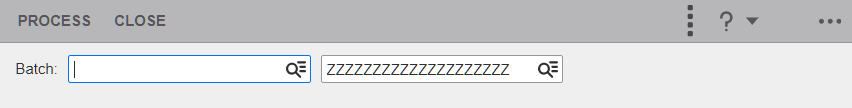
\includegraphics[width=0.8\textwidth]{Immagini/Sessioni/ExecuteBatchRuns_txamg3200m000}
	\caption{Sessione di Esecuzione Batch (txamg3200m000)}
	\label{fig:sessione_esecuzione_batch}
\end{figure}

I \textit{Runs Errors} offrono un riscontro immediato di blocchi logici o semantici.
Sono stati eseguiti scenari in cui la validazione è forzata per respingere record privi di riferimenti chiave,
verificando che la linea errata fosse elaborata senza però interromperne il caricamento dell'intero \textit{Run}.

\begin{figure}[H]
	\centering
	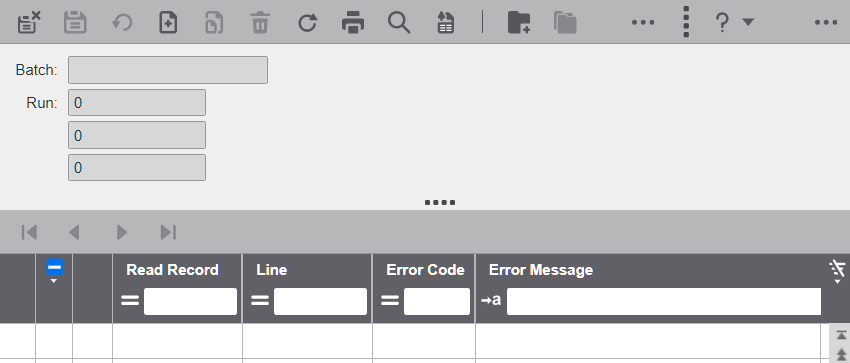
\includegraphics[width=0.8\textwidth]{Immagini/Sessioni/RunsErrors_txamg3503m000}
	\caption{Dettaglio degli errori di migrazione (txamg3503m000)}
	\label{fig:dettaglio_errori_migrazione}
\end{figure}

Gli errori segnalati sono dettagliati all'interno della tabella \texttt{txamg303}, le cui colonne principali permettono
di investigare quale linea e record sia fallito:
\begin{itemize}
    \item \texttt{runs}: Identificativo del Run
    \item \texttt{rere}: Riga di lettura (\textit{Read Record})
    \item \texttt{line}: Riga testuale all'interno del file sorgente
    \item \texttt{errc}: Codice specifico dell'errore (\textit{Error Code})
    \item \texttt{errm}: Descrizione del problema riscontrato dal DAL (\textit{Error Message})
\end{itemize}

Oltre ai controlli manuali, questo tracciamento funge da base per le strategie di \textit{retry} o per
le \textit{sanity check} del dato prima della re-immissione: individuando la tipologia di errore, il consulente o l'operatore
può decidere se modificarne il mapping, apportare modifiche sul file d'origine o creare estensioni
specifiche ai moduli generati dal tool.

\section{Verifica dell'Integrità dei Dati}
\subsection{Matching tra Dati Sorgente (Legacy) e Destinazione (Cloud)}
Ogni file migrato viene tracciato sulle tabelle atte al monitoraggio (\texttt{txamg301}, \texttt{txamg302}). Il \textit{matching}
prevede che vengano comparati il numero dei record letti, processati ed eventualmente respinti rispetto all'origine.
Questo consente di ottenere la garanzia del risultato atteso, in quanto una discrepanza nel numero di dati letti e scritti,
segnalerebbe un errore evidente.

Nello specifico la tabella \texttt{txamg301} incapsula le metriche di base del processo:
\begin{longtable}{@{} l p{4cm} p{7cm} @{}}
    \toprule
    \textbf{Campo} & \textbf{Nome} & \textbf{Descrizione} \\
    \midrule
    \endfirsthead
    \toprule
    \textbf{Campo} & \textbf{Nome} & \textbf{Descrizione} \\
    \midrule
    \endhead
    \midrule
    \multicolumn{3}{r}{{Continua nella pagina successiva}} \\
    \bottomrule
    \endfoot
    \bottomrule
    \caption{Struttura dei conteggi per l'affidabilità (txamg301)}
    \endlastfoot
    \texttt{rere} & Records Read & Il volume totale delle istruzioni e record processati dal tool \\
    \texttt{repr} & Record Processed & Quanti dei record immessi hanno dato esito positivo dopo tutti i trigger \\
    \texttt{reer} & Records Discarded & Numero di istanze rifiutate o bloccate dal check del DB \\
\end{longtable}

I report prodotti (tramite moduli ad hoc come \texttt{txamgdll0011} per il log d'errore) forniscono la garanzia
numerica dell'operazione, permettendo al team di validazione di avere stime certe prima dell'import su CloudSuite finale.

Questo approccio garantisce che le disconnessioni di rete o i blocchi temporanei non lascino i dati in uno stato di
incertezza.
Il tool si comporta in maniera deterministica e produce riscontri sempre validati rispetto al totale.

\begin{figure}[H]
	\centering
	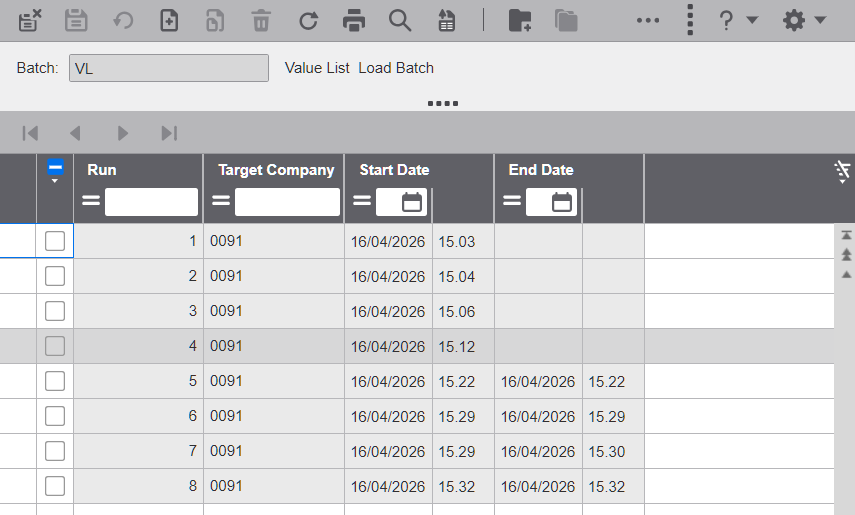
\includegraphics[width=0.8\textwidth]{Immagini/Sessioni/RunsByBatch_txamg3500m000}
	\caption{Storico e validazione delle esecuzioni (txamg3500m000)}
	\label{fig:storico_validazione_runs}
\end{figure}

%! Author = gabry
%! Date = 03/07/2026

\chapter{Conclusioni}\label{ch:conclusioni}

% \appendix
% \chapter{Dettaglio della Struttura delle Tabelle}
\label{appendix:tabelle}

Viene qui riportata la struttura dettagliata delle tabelle progettate, sviluppate e utilizzate all'interno del Migration Tool.
Ogni tabella è identificata da un codice univoco con prefisso \texttt{txamg}.
Ove le prime due lettere (\texttt{tx}) indicano il package \textit{custom}, le successive tre lettere (\texttt{amg}) rappresentano il modulo).

\section{Tabelle di Configurazione e Metadati}

\begin{longtable}{@{} l l l r p{6cm} @{}}
\caption{Struttura della tabella txamg000 (Parametri Generali)} \label{tab:txamg000} \\
\toprule
\textbf{Campo} & \textbf{Dominio} & \textbf{Tipo Dato} & \textbf{Lung.} & \textbf{Descrizione} \\
\midrule
\endfirsthead
\multicolumn{5}{c}%
{{\bfseries \tablename\ \thetable{} -- Continua dalla pagina precedente}} \\
\toprule
\textbf{Campo} & \textbf{Dominio} & \textbf{Tipo Dato} & \textbf{Lung.} & \textbf{Descrizione} \\
\midrule
\endhead
\midrule
\multicolumn{5}{r}{{Continua nella pagina successiva}} \\
\bottomrule
\endfoot
\bottomrule
\endlastfoot
indt & tc date & UTC Date/Time & 22 & Introduction Date \\
dsca & tc mcs.str50m & Multibyte String & 50 & Description \\
lopk & tx amg.cpac & String & 2 & Load Library Package \\
lomd & tx amg.cmod & String & 3 & Load Library Module \\
loff & tc mcs.long & Long & 10 & Load Library First Free Number \\
prpk & tx amg.cpac & String & 2 & Process Library Package \\
prmd & tx amg.cmod & String & 3 & Process Library Module \\
prff & tc mcs.long & Long & 10 & Process Library First Free Number \\
bpat & tc path2 & String & 128 & Base Path for Files \\
\end{longtable}

\begin{longtable}{@{} l l l r p{6cm} @{}}
\caption{Struttura della tabella txamg100 (Gruppi Tabelle)} \label{tab:txamg100} \\
\toprule
\textbf{Campo} & \textbf{Dominio} & \textbf{Tipo Dato} & \textbf{Lung.} & \textbf{Descrizione} \\
\midrule
\endfirsthead
\caption[]{Struttura della tabella txamg100 (Gruppi Tabelle) -- Continua} \\
\toprule
\textbf{Campo} & \textbf{Dominio} & \textbf{Tipo Dato} & \textbf{Lung.} & \textbf{Descrizione} \\
\midrule
\endhead
grou & tx amg.grou & String & 20 & Table Group \\
dsca & tc dsca & Multibyte String & 30 & Description \\
bpat & tc path2 & String & 128 & Subfolder \\
\end{longtable}

\begin{longtable}{@{} l l l r p{6cm} @{}}
\caption{Struttura della tabella txamg110 (Data Files)} \label{tab:txamg110} \\
\toprule
\textbf{Campo} & \textbf{Dominio} & \textbf{Tipo Dato} & \textbf{Lung.} & \textbf{Descrizione} \\
\midrule
\endfirsthead
\caption[]{Struttura della tabella txamg110 (Data Files) -- Continua} \\
\toprule
\textbf{Campo} & \textbf{Dominio} & \textbf{Tipo Dato} & \textbf{Lung.} & \textbf{Descrizione} \\
\midrule
\endhead
grou & tx amg.grou & String & 20 & Table Group \\
dfil & tx amg.dfil & String & 20 & Data File \\
dsca & tc dsca & Multibyte String & 30 & Description \\
fast & tx amg.fast & Enumerated & 10 & File Type \\
sepa & tc mcs.str1 & String & 1 & Separator \\
frzn & tc yesno & Enumerated & 5 & Frozen \\
cprs & tx amg.cprs & String & 9 & Load Library \\
cpac & tx amg.cpac & String & 2 & Ref Table Package \\
cmod & tx amg.cmod & String & 3 & Ref Table Module \\
flno & tx amg.flno & String & 3 & Ref Table \\
mufi & tc yesno & Enumerated & 5 & Multifile Datafile \\
bpat & tc path2 & String & 128 & Subfolder \\
\end{longtable}

\begin{longtable}{@{} l l l r p{6cm} @{}}
\caption{Struttura della tabella txamg111 (Campi Data File)} \label{tab:txamg111} \\
\toprule
\textbf{Campo} & \textbf{Dominio} & \textbf{Tipo Dato} & \textbf{Lung.} & \textbf{Descrizione} \\
\midrule
\endfirsthead
\caption[]{Struttura della tabella txamg111 (Campi Data File) -- Continua} \\
\toprule
\textbf{Campo} & \textbf{Dominio} & \textbf{Tipo Dato} & \textbf{Lung.} & \textbf{Descrizione} \\
\midrule
\endhead
grou & tx amg.grou & String & 20 & Table Group \\
dfil & tx amg.dfil & String & 20 & Data File \\
fdno & tx amg.fdno & Integer & 4 & Field Number \\
fdnm & tx amg.dfnm & String & 20 & Field Name \\
dsca & tc dsca & Multibyte String & 30 & Description \\
stpn & tx amg.fdno & Integer & 4 & Start Position \\
leng & tx amg.fdno & Integer & 4 & Length \\
atyp & tx amg.atyp & Enumerated & 10 & Dafile Field Type \\
adgb & tc mcs.int & Integer & 3 & Digits Before \\
adga & tc mcs.int & Integer & 3 & Digits After \\
cpac & tx amg.cpac & String & 2 & Ref Table Package \\
cmod & tx amg.cmod & String & 3 & Ref Table Module \\
flno & tx amg.flno & String & 3 & Ref Table \\
rfnm & tx amg.fdnm & String & 8 & Ref Field Name \\
\end{longtable}

\section{Tabelle di Mapping e Logica}

\begin{longtable}{@{} l l l r p{6cm} @{}}
\caption{Struttura della tabella txamg200 (Batch)} \label{tab:txamg200} \\
\toprule
\textbf{Campo} & \textbf{Dominio} & \textbf{Tipo Dato} & \textbf{Lung.} & \textbf{Descrizione} \\
\midrule
\endfirsthead
\caption[]{Struttura della tabella txamg200 (Batch) -- Continua} \\
\toprule
\textbf{Campo} & \textbf{Dominio} & \textbf{Tipo Dato} & \textbf{Lung.} & \textbf{Descrizione} \\
\midrule
\endhead
cbat & tx amg.cbat & String & 20 & Batch \\
dsca & tc dsca & Multibyte String & 30 & Description \\
bpat & tc path2 & String & 128 & Subfolder \\
\end{longtable}

\begin{longtable}{@{} l l l r p{6cm} @{}}
\caption{Struttura della tabella txamg201 (Sequenza Batch)} \label{tab:txamg201} \\
\toprule
\textbf{Campo} & \textbf{Dominio} & \textbf{Tipo Dato} & \textbf{Lung.} & \textbf{Descrizione} \\
\midrule
\endfirsthead
\caption[]{Struttura della tabella txamg201 (Sequenza Batch) -- Continua} \\
\toprule
\textbf{Campo} & \textbf{Dominio} & \textbf{Tipo Dato} & \textbf{Lung.} & \textbf{Descrizione} \\
\midrule
\endhead
cbat & tx amg.cbat & String & 20 & Batch \\
sequ & tc mcs.int & Integer & 3 & Seq. \\
grou & tx amg.grou & String & 20 & Table Group \\
dfil & tx amg.dfil & String & 20 & Data File \\
migt & tx amg.migt & Enumerated & 10 & Migration Type \\
cprs & tx amg.cprs & String & 9 & Process Library \\
ilgn & tx amg.logn & String & 8 & Internal Owner \\
elgn & tx amg.logn & String & 8 & External Owner \\
txta & tc txtn & Text & 0 & Notes \\
frzn & tc yesno & Enumerated & 5 & Frozen \\
\end{longtable}

\begin{longtable}{@{} l l l r p{6cm} @{}}
\caption{Struttura della tabella txamg202 (Tabelle di Destinazione)} \label{tab:txamg202} \\
\toprule
\textbf{Campo} & \textbf{Dominio} & \textbf{Tipo Dato} & \textbf{Lung.} & \textbf{Descrizione} \\
\midrule
\endfirsthead
\caption[]{Struttura della tabella txamg202 (Tabelle di Destinazione) -- Continua} \\
\toprule
\textbf{Campo} & \textbf{Dominio} & \textbf{Tipo Dato} & \textbf{Lung.} & \textbf{Descrizione} \\
\midrule
\endhead
cbat & tx amg.cbat & String & 20 & Batch \\
sequ & tc mcs.int & Integer & 3 & Seq. \\
sseq & tc mcs.int & Integer & 3 & SubSeq. \\
cpac & tx amg.cpac & String & 2 & Package \\
cmod & tx amg.cmod & String & 3 & Module \\
flno & tx amg.flno & String & 3 & Table \\
flnm & tc dsca & Multibyte String & 30 & Table Name \\
ilgn & tx amg.logn & String & 8 & Internal Owner \\
elgn & tx amg.logn & String & 8 & External Owner \\
shrd & tc yesno & Enumerated & 5 & Shared \\
udal & tc yesno & Enumerated & 5 & Use DAL \\
utyp & tx amg.utyp & Enumerated & 10 & DB Operation \\
txta & tc txtn & Text & 0 & Functional Notes \\
\end{longtable}

\begin{longtable}{@{} l l l r p{6cm} @{}}
\caption{Struttura della tabella txamg203 (Campi Mappati)} \label{tab:txamg203} \\
\toprule
\textbf{Campo} & \textbf{Dominio} & \textbf{Tipo Dato} & \textbf{Lung.} & \textbf{Descrizione} \\
\midrule
\endfirsthead
\caption[]{Struttura della tabella txamg203 (Campi Mappati) -- Continua} \\
\toprule
\textbf{Campo} & \textbf{Dominio} & \textbf{Tipo Dato} & \textbf{Lung.} & \textbf{Descrizione} \\
\midrule
\endhead
cbat & tx amg.cbat & String & 20 & Batch \\
sequ & tc mcs.int & Integer & 3 & Seq. \\
sseq & tc mcs.int & Integer & 3 & SubSeq. \\
cpac & tx amg.cpac & String & 2 & Package \\
cmod & tx amg.cmod & String & 3 & Module \\
flno & tx amg.flno & String & 3 & Table \\
fdno & tx amg.fdno & Integer & 4 & Field N. \\
fdnm & tx amg.fdnm & String & 8 & Field Name \\
icdf & tc yesno & Enumerated & 5 & CDF \\
isml & tc yesno & Enumerated & 5 & ML \\
fdsc & tc dsca & Multibyte String & 30 & Field Desc \\
comb & tc yesno & Enumerated & 5 & Comb. \\
pacd & tx amg.cpac & String & 2 & Domain Package \\
cdom & tx amg.cdom & String & 12 & Domain \\
type & tx amg.type & Enumerated & 10 & Data Type \\
digb & tc mcs.int & Integer & 3 & Digit Before \\
diga & tc mcs.int & Integer & 3 & Digit After \\
iniv & tc dsca & Multibyte String & 30 & Initial Value \\
mand & tc yesno & Enumerated & 5 & Mandatory \\
rfpa & tx amg.cpac & String & 2 & Ref. Table Package \\
rfmo & tx amg.cmod & String & 3 & Ref. Table Module \\
rffn & tx amg.cmod & String & 3 & Ref. Table \\
rffd & tx amg.fdnm & String & 8 & Ref. Field \\
dept & tc mcs.int & Integer & 3 & Depth \\
\end{longtable}

\section{Tabelle di Esecuzione e Log}

\begin{longtable}{@{} l l l r p{6cm} @{}}
\caption{Struttura della tabella txamg300 (Run di Esecuzione)} \label{tab:txamg300} \\
\toprule
\textbf{Campo} & \textbf{Dominio} & \textbf{Tipo Dato} & \textbf{Lung.} & \textbf{Descrizione} \\
\midrule
\endfirsthead
\caption[]{Struttura della tabella txamg300 (Run di Esecuzione) -- Continua} \\
\toprule
\textbf{Campo} & \textbf{Dominio} & \textbf{Tipo Dato} & \textbf{Lung.} & \textbf{Descrizione} \\
\midrule
\endhead
cbat & tx amg.cbat & String & 20 & Batch \\
runs & tc mcs.long & Long & 10 & Run \\
ncmp & tc ncmp & Integer & 4 & Target Company \\
stdt & tc date & UTC Date/Time & 22 & Start Date \\
endt & tc date & UTC Date/Time & 22 & End Date \\
\end{longtable}

\begin{longtable}{@{} l l l r p{6cm} @{}}
\caption{Struttura della tabella txamg301 (Log Esecuzione per Batch)} \label{tab:txamg301} \\
\toprule
\textbf{Campo} & \textbf{Dominio} & \textbf{Tipo Dato} & \textbf{Lung.} & \textbf{Descrizione} \\
\midrule
\endfirsthead
\caption[]{Struttura della tabella txamg301 (Log Esecuzione per Batch) -- Continua} \\
\toprule
\textbf{Campo} & \textbf{Dominio} & \textbf{Tipo Dato} & \textbf{Lung.} & \textbf{Descrizione} \\
\midrule
\endhead
cbat & tx amg.cbat & String & 20 & Batch \\
runs & tc mcs.long & Long & 10 & Run \\
sequ & tc mcs.long & Long & 10 & Sequence \\
stdt & tc date & UTC Date/Time & 22 & Start Date \\
endt & tc date & UTC Date/Time & 22 & End Date \\
rere & tc mcs.long & Long & 10 & Records Read \\
repr & tc mcs.long & Long & 10 & Record Processed \\
reer & tc mcs.long & Long & 10 & Records Discarded \\
\end{longtable}

\begin{longtable}{@{} l l l r p{6cm} @{}}
\caption{Struttura della tabella txamg302 (Log Esecuzione per SubSeq)} \label{tab:txamg302} \\
\toprule
\textbf{Campo} & \textbf{Dominio} & \textbf{Tipo Dato} & \textbf{Lung.} & \textbf{Descrizione} \\
\midrule
\endfirsthead
\caption[]{Struttura della tabella txamg302 (Log Esecuzione per SubSeq) -- Continua} \\
\toprule
\textbf{Campo} & \textbf{Dominio} & \textbf{Tipo Dato} & \textbf{Lung.} & \textbf{Descrizione} \\
\midrule
\endhead
cbat & tx amg.cbat & String & 20 & Batch \\
runs & tc mcs.long & Long & 10 & Run \\
sequ & tc mcs.long & Long & 10 & Sequence \\
sseq & tc mcs.long & Long & 10 & Subsequence \\
stdt & tc date & UTC Date/Time & 22 & Start Date \\
endt & tc date & UTC Date/Time & 22 & End Date \\
\end{longtable}

\begin{longtable}{@{} l l l r p{6cm} @{}}
\caption{Struttura della tabella txamg303 (Errori di Esecuzione)} \label{tab:txamg303} \\
\toprule
\textbf{Campo} & \textbf{Dominio} & \textbf{Tipo Dato} & \textbf{Lung.} & \textbf{Descrizione} \\
\midrule
\endfirsthead
\caption[]{Struttura della tabella txamg303 (Errori di Esecuzione) -- Continua} \\
\toprule
\textbf{Campo} & \textbf{Dominio} & \textbf{Tipo Dato} & \textbf{Lung.} & \textbf{Descrizione} \\
\midrule
\endhead
cbat & tx amg.cbat & String & 20 & Batch \\
runs & tc mcs.long & Long & 10 & Run \\
sequ & tc mcs.long & Long & 10 & Sequence \\
sseq & tc mcs.long & Long & 10 & Subsequence \\
rere & tc mcs.long & Long & 10 & Read Record \\
line & tc mcs.long & Long & 10 & Line \\
errc & tc mcs.int & Integer & 3 & Error Code \\
errm & tc mcs.s999m & Multibyte String & 999 & Error Message \\
\end{longtable}




% ----------------------
% ---- BIBLIOGRAPHY ----
% ----------------------
\backmatter
\sloppy % serve a non far andare i link oltre ai margini
\printbibliography[nottype=online, heading=bibintoc, title=Bibliografia]
\printbibliography[type=online, heading=bibintoc, title=Sitografia]

% ----------------------
% ---- DOCUMENT END ----
% ----------------------
\end{document} % Fine documento